%*************************************************************************************************************************
\section{Uncertainty Quantification in Nuclear Engineering Thermal-Hydraulics}\label{sec:intro_uncertainty_quantification}
%*************************************************************************************************************************

% Introductory Paragraph
Before continuing the discussion of uncertainty analysis of code predictions, it will be worthwhile to define some additional terminologies to avoid later confusion.

In making a connection with the notion of simulator \emph{simulator} introduced in Section~\ref{sec:intro_computer_simulation}, 
recall that from Fig.~\ref{fig:ch1_th_system_code} \emph{input deck} and the code itself are distinct elements.
Fig.~\ref{fig:ch1_simulator_io} depicts the notion of simulator of a thermal-hydraulics system in a more generic way, as an input/output model.
\begin{figure}[bth]	
	\centering
	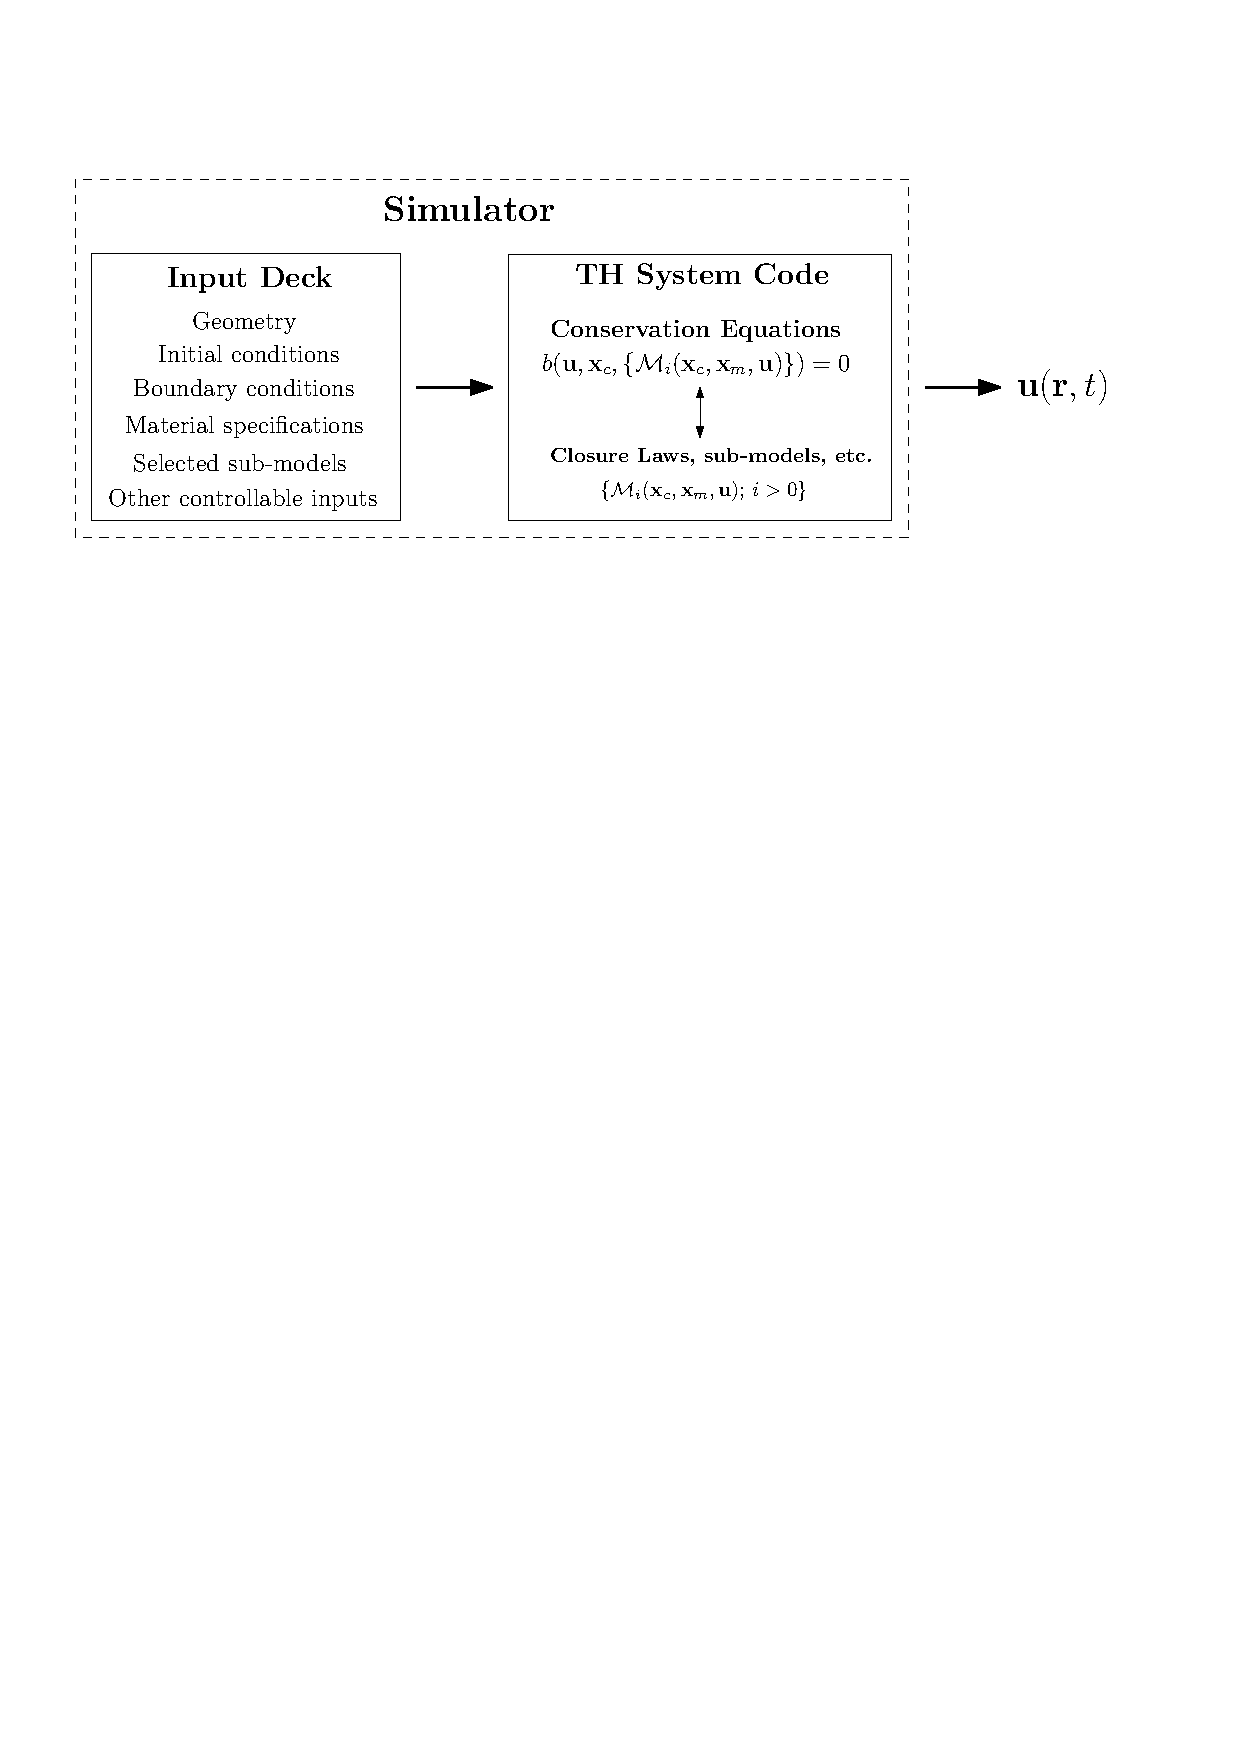
\includegraphics[width=\textwidth]{../figures/chapter1/figures/simulator_io}
	\caption[Simplified illustration of a simulator as an input/output model]{Simplified illustration of a simulator as an input/output model.}
	\label{fig:ch1_simulator_io}
\end{figure}

Indeed input deck defines specific problem (i.e., system) of interest.
It includes the specifications for geometrical configuration (i.e., the nodalization), choice of material and fluid involves, as well as initial and boundary conditions.
It may also include the setting for the numerical solver.
Some of those specifications (such as the boundary conditions, etc.) are parametrized and constitutes \emph{controllable inputs} denoted by $\bm{x}_c$. 
Specifying the input deck, as far as user is concerned, completely defines the problem and the code will solve the conservation equations which output the dynamic state of relevant physical variables $\mathbf{u}(\bm{r}, t)$ (e.g., fluid pressure, temperature, wall temperature, etc.).
The conservation equations are closed with additional set of closure laws (and other sub-models) $\mathcal{M}_i(\bm{x}_c, \bm{x}_m, \bm{u})$.
These closure laws are, in turn, parametrized with a set of model specific parameters denoted by $\bm{x}_m$.
This set of parameters is referred to as the \emph{physical model parameters}.

%----------------------------------------------------------------------------------------------
\subsection{Statistical Uncertainty Analysis}\label{sub:intro_statistical_uncertainty_analysis}
%----------------------------------------------------------------------------------------------

% Best-estimate, limitation
As explained, best-estimate analysis uses more realistic modeling assumptions for analyzing transient behavior of \gls[hyper=false]{npp}.
It attempts as realistically as possible to describe the behavior of the relevant physical processes occur during the plant transient.
And yet, even the best available understanding of the physical process is still limited.
Understanding of complex phenomena might not yet adequate and data support for some processes can be very limited.
Simplifying assumptions, approximations, and expert judgments to some degree are unavoidable and still required to have a complete analysis.

% Best-estimate, plus uncertainty
Hence, best-estimate analysis has to be complemented with uncertainty analysis.
The ultimate goal of uncertainty analysis is to associate code prediction with its uncertainty.
These combined quantities are then compared with certain regulator safety limits (e.g., \gls[hyper=false]{pct}) to check whether the limits still fall outside the uncertainty band of the code prediction.

% Source of possible uncertainties

% Statistical uncertainty analysis, Inputs as random variables 

% Source of uncertainty, initial and boundary condition

% Source of uncertainty, physical model parameters

% Inverse uncertainty

% Connection to PREMIUM Benchmark

%---------------------------------------------------------------
\subsection{OECD/NEA PREMIUM Benchmark}\label{sub:intro_premium}
%---------------------------------------------------------------

% Introductory paragraph
The \gls[hyper=false]{premium} benchmark was an activity launched by the \gls[hyper=false]{oecd}/\gls[hyper=false]{nea} in $2012$ and concluded in $2016$ with the aim to advance the methods for quantifying the uncertainties associated with the physical model parameters in \gls[hyper=false]{th} system codes.
It was the continuation of the previous project \gls[hyper=false]{bemuse}, which concetrated on the propagation and sensitivity analysis of the input uncertainties in large scale simulation (large break \gls[hyper=false]{loca}).
The main finding of \gls[hyper=false]{bemuse} can be found in \cite{Perez2011}.
The emphasis of the \gls[hyper=false]{premium} benchmark was placed on the derivation of the model parameters uncertainty and their validation.

% Scope of the Project

% Main Findings

%-------------------------------------------------------
\subsection{GRS Methodology}\label{sub:intro_grs_method}
%-------------------------------------------------------

%-----------------------------------------------------------
\subsection{FFTBM Methodology}\label{sub:intro_fftbm_method}
%-----------------------------------------------------------

%-------------------------------------------------------
\subsection{CIRC\'E}\label{sub:intro_circe_method}
%-------------------------------------------------------
